
%(BEGIN_QUESTION)
% Copyright 2014, Tony R. Kuphaldt, released under the Creative Commons Attribution License (v 1.0)
% This means you may do almost anything with this work of mine, so long as you give me proper credit

A special type of AC generator called a {\it self-excited induction generator} may be constructed from a bank of capacitors and a standard three-phase induction motor like this:

$$\includegraphics[width=15.5cm]{i03311x01.eps}$$

Assuming $V_A$ measures 248 volts at an angle of $-15^o$ (compared to some other reference defined as zero degrees), calculate the magnitude and phase angle of the current through the capacitor connected to phase B (connected to motor terminal T2).  Assume a frequency of 60 Hz and an ABC phase rotation:

\vskip 10pt

$I$ = \underbar{\hskip 80pt}

\underbar{file i03311}
%(END_QUESTION)





%(BEGIN_ANSWER)

$I$ = 1.870 A $\angle$ $-45^o$ or 1.870 A $\angle$ $315^o$

%(END_ANSWER)





%(BEGIN_NOTES)


%(END_NOTES)


